\documentclass{article}
\usepackage[utf8]{inputenc}
\usepackage{amsmath}
\usepackage{amsfonts}
\usepackage{mathrsfs}
\usepackage{graphicx}
\usepackage{subcaption}
\usepackage[top=20truemm,bottom=20truemm,left=20truemm,right=20truemm]{geometry}

\title{Chaotic Dynamics: Homework 1}
\author{Kansuke Ikehara (Kansuke.Ikehara@colorado.edu)}

\begin{document}
\maketitle

\subsection*{Problem 1}
I have implemented the simple box-counting algorithm using a three-dimensional array. It basically scans the trajectory and puts "1" onto the corresponding array element for each point of the trajectory. It thens counts the number of "1"s in the array.

\subsection*{Problem 2}
\subsubsection*{(a)}
Figure \ref{q2a} shows a plot of $\log N(\epsilon)$ versus $\log (\frac{1}{\epsilon})$. Smaller values of $\epsilon$ could not be used for calculation as it would run out of the memory. The shape of the plot is linear, which makes sense since we expect the power-law scaling in the log-log plot. We would have seen flat zones on both sides of the plot if we calculated $\log N(\epsilon)$ for larger and smaller $\epsilon$s.

\begin{figure}[h]
  \centering
  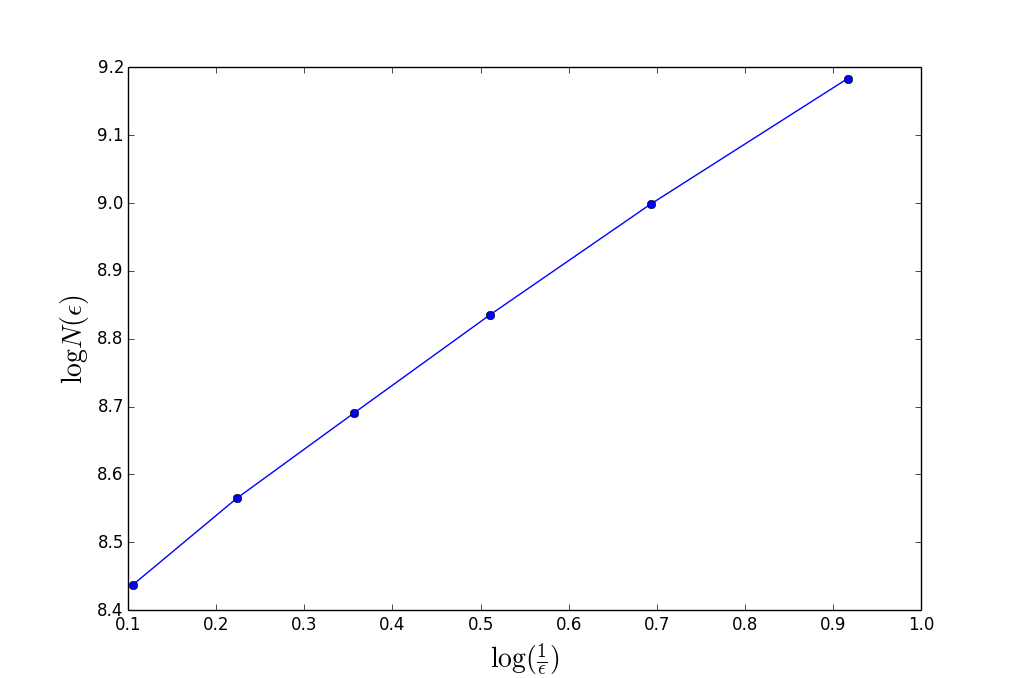
\includegraphics[height=1.5in]{figs/q2_a.png}
  \caption{$\log N(\epsilon)$ versus $\log (\frac{1}{\epsilon})$.}
  \label{q2a}
\end{figure}

\subsubsection*{(b)}
Figure \ref{q2b} shows plots of $\log N(\epsilon)$ versus $\log (\frac{1}{\epsilon})$ for both normal-length and long-length trajectories. The plot for longer one is obviously above the other one, as it contains more points thus more boxes to cover the attractor. The slope of the plot is slightly higher than the normal-length one as well. Since longer trajectory is close to the true shape of the attractor, we should trust the result from it.

\begin{figure}[h]
  \centering
  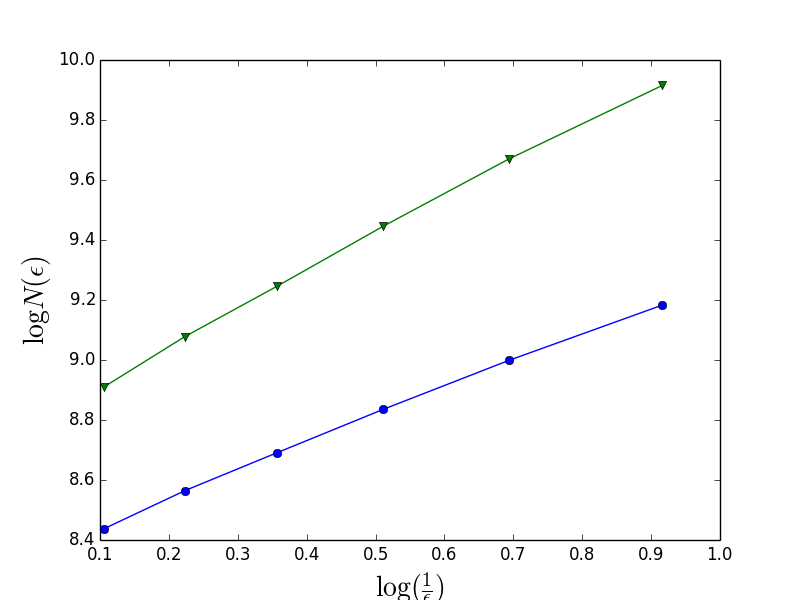
\includegraphics[height=2in]{figs/q2_b.png}
  \caption{Plots of $\log N(\epsilon)$ versus $\log (\frac{1}{\epsilon})$ for both trajectories. The one above corresponds to the longer trajectory.}
  \label{q2b}
\end{figure}

\subsubsection*{(c)}
Figure \ref{q2c} shows plots of $\log N(\epsilon)$ versus $\log (\frac{1}{\epsilon})$ for three trajectories we have had so far including the reconstructed one for this problem. Embedding dimension is $m = 3$. The bottom line in the plot corresponds to the reconstructed one, which seems to have the almost same slope as other two, but the $\log N(\epsilon)$ is lower. This is due to the fact that we have fewer points in the reconstructed state-space.

\begin{figure}[h]
  \centering
  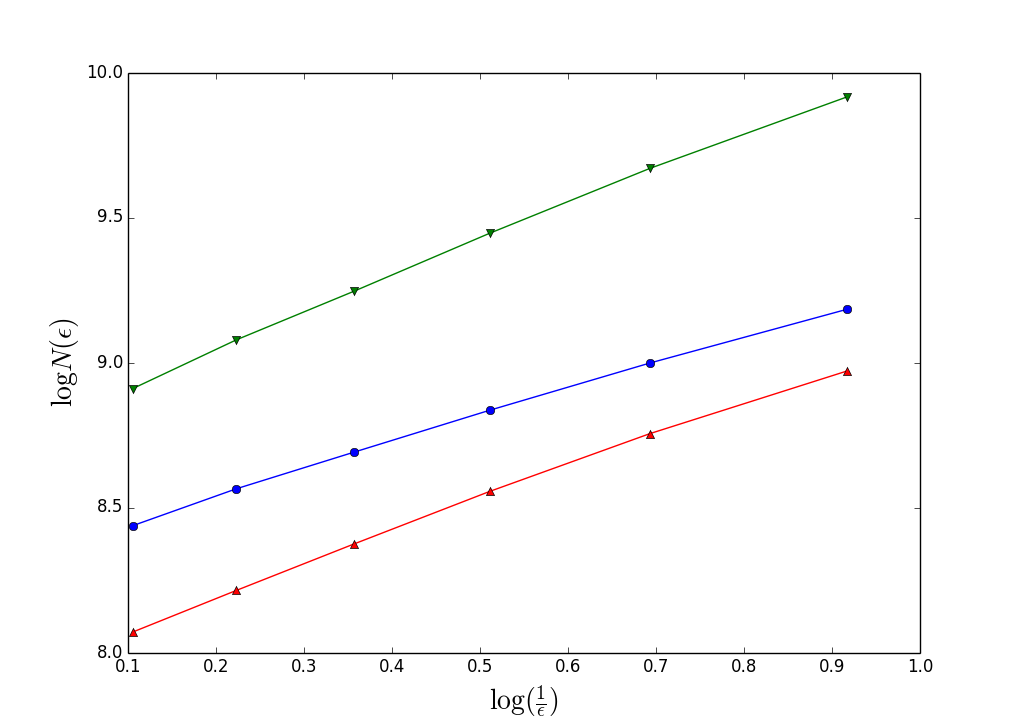
\includegraphics[height=1.5in]{figs/q2_c.png}
  \caption{Plots of $\log N(\epsilon)$ versus $\log (\frac{1}{\epsilon})$ for three trajectories (problems (a), (b) and (c)).}
  \label{q2c}
\end{figure}

\subsection*{Problem 3}
One possible way to alleviate the memory limitation is to use a sparse matrix for storing the "1"s for checking if a point is in a box or not. Since most of the entries in the matrix is 0s, they consume a lot of memory space unnecessarily. If we could "compress" the entries for 0s, it would save memory space and lead to faster computation.

\subsection*{Problem 4}
Figures \ref{q4_c} and \ref{q4_d} show $C(m, \epsilon)$ versus $\epsilon$, and $D(m, \epsilon)$ versus $\epsilon$, respectively. The plot for $C(m, \epsilon)$ shows a power-law like straight line around $\epsilon = 10^0$. The correlation dimension $D(m, \epsilon)$ for that region seems plateau-like structure with some noise. We could say from this plot of $D(m, \epsilon)$ that the correlation dimension of the reconstructed trajectory is around 2.


\begin{figure}
\centering
\begin{subfigure}{.5\textwidth}
  \centering
  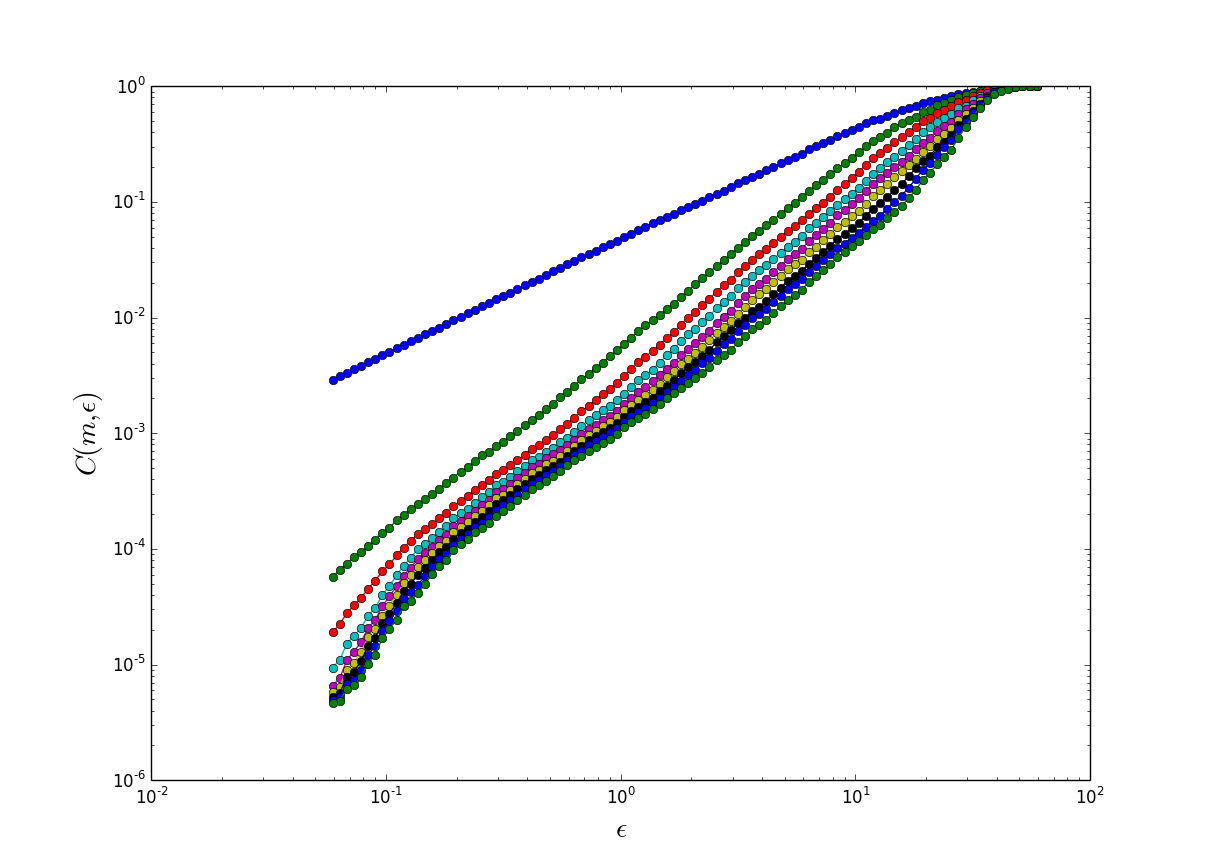
\includegraphics[height=2in]{figs/q4_c.png}
  \caption{$C(m, \epsilon)$ versus $\epsilon$}
  \label{q4_c}
\end{subfigure}%
\begin{subfigure}{.5\textwidth}
  \centering
  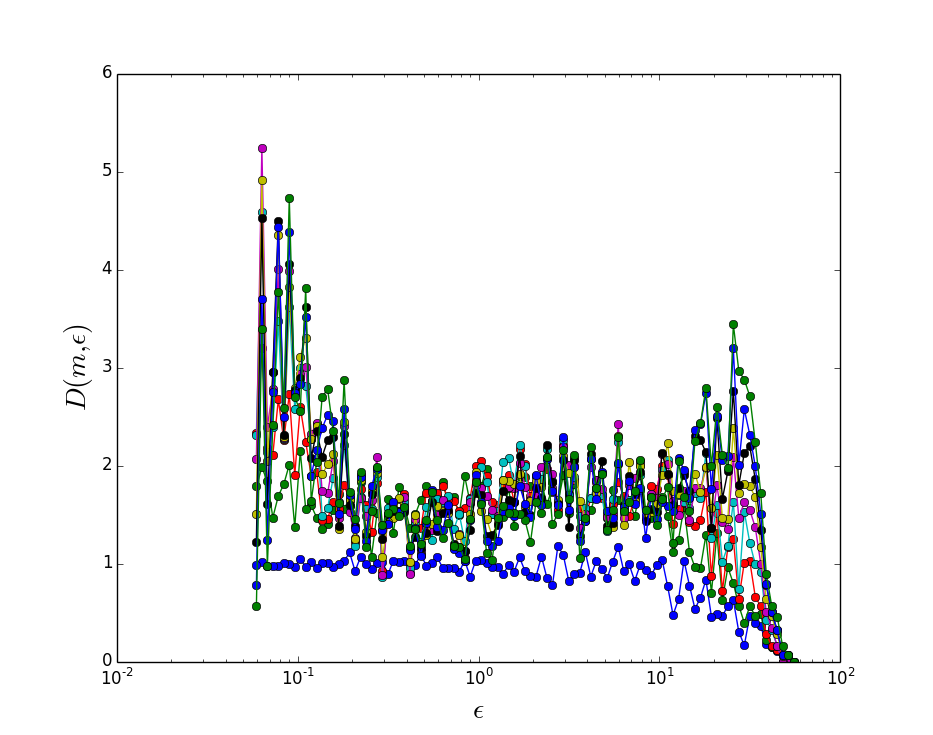
\includegraphics[height=2in]{figs/q4_d.png}
  \caption{$D(m, \epsilon)$ versus $\epsilon$}
  \label{q4_d}
\end{subfigure}
\caption{}
\label{q4}
\end{figure}

\end{document}












